%%%%%%%%%%%%%%%%%%%%%%%%%%%%%%%%%%%%%%%%%%%%%%%%%%%%%%%%%%%%%%%%%%%%%%%%%%%%%
%
%  System        : 
%  Module        : 
%  Object Name   : $RCSfile$
%  Revision      : $Revision$
%  Date          : $Date$
%  Author        : $Author$
%  Created By    : Robert Heller
%  Created       : Wed Nov 16 09:06:35 2022
%  Last Modified : <221116.0907>
%
%  Description 
%
%  Notes
%
%  History
% 
%%%%%%%%%%%%%%%%%%%%%%%%%%%%%%%%%%%%%%%%%%%%%%%%%%%%%%%%%%%%%%%%%%%%%%%%%%%%%
%
%    Copyright (C) 2022  Robert Heller D/B/A Deepwoods Software
%			51 Locke Hill Road
%			Wendell, MA 01379-9728
%
%    This program is free software; you can redistribute it and/or modify
%    it under the terms of the GNU General Public License as published by
%    the Free Software Foundation; either version 2 of the License, or
%    (at your option) any later version.
%
%    This program is distributed in the hope that it will be useful,
%    but WITHOUT ANY WARRANTY; without even the implied warranty of
%    MERCHANTABILITY or FITNESS FOR A PARTICULAR PURPOSE.  See the
%    GNU General Public License for more details.
%
%    You should have received a copy of the GNU General Public License
%    along with this program; if not, write to the Free Software
%    Foundation, Inc., 675 Mass Ave, Cambridge, MA 02139, USA.
%
% 
%
%%%%%%%%%%%%%%%%%%%%%%%%%%%%%%%%%%%%%%%%%%%%%%%%%%%%%%%%%%%%%%%%%%%%%%%%%%%%%

\documentclass[12pt,twoside]{article}
\usepackage{graphicx}
\usepackage{mathptm}
\usepackage{times}
\usepackage{makeidx}
\usepackage{ifpdf}
\usepackage{footmisc}
\ifpdf 
\usepackage[pdftex,
            pagebackref=true,
            colorlinks=true,
            linkcolor=blue,
            unicode
           ]{hyperref}
\else
\usepackage[ps2pdf,
            pagebackref=true,
            colorlinks=true,
            linkcolor=blue,
            unicode
           ]{hyperref}
\usepackage{pspicture}
\fi
\usepackage{url}
\pagestyle{headings}
\makeindex
\emergencystretch=50pt
\setcounter{tocdepth}{3}
\setcounter{secnumdepth}{3}
\title{PocketBeagle Command Station Instructions}
\author{Robert Heller \\ The Country Robot \\ Wendell, MA, USA}
\date{\today}
\newcommand{\chapter}[1]{}
\begin{document}
\maketitle
\tableofcontents
\listoffigures
\clearpage
\section*{Introduction}
%%%%%%%%%%%%%%%%%%%%%%%%%%%%%%%%%%%%%%%%%%%%%%%%%%%%%%%%%%%%%%%%%%%%%%%%%%%%%
%
%  System        : 
%  Module        : 
%  Object Name   : $RCSfile$
%  Revision      : $Revision$
%  Date          : $Date$
%  Author        : $Author$
%  Created By    : Robert Heller
%  Created       : Wed Nov 16 09:04:20 2022
%  Last Modified : <221116.1434>
%
%  Description 
%
%  Notes
%
%  History
% 
%%%%%%%%%%%%%%%%%%%%%%%%%%%%%%%%%%%%%%%%%%%%%%%%%%%%%%%%%%%%%%%%%%%%%%%%%%%%%
%
%    Copyright (C) 2022  Robert Heller D/B/A Deepwoods Software
%			51 Locke Hill Road
%			Wendell, MA 01379-9728
%
%    This program is free software; you can redistribute it and/or modify
%    it under the terms of the GNU General Public License as published by
%    the Free Software Foundation; either version 2 of the License, or
%    (at your option) any later version.
%
%    This program is distributed in the hope that it will be useful,
%    but WITHOUT ANY WARRANTY; without even the implied warranty of
%    MERCHANTABILITY or FITNESS FOR A PARTICULAR PURPOSE.  See the
%    GNU General Public License for more details.
%
%    You should have received a copy of the GNU General Public License
%    along with this program; if not, write to the Free Software
%    Foundation, Inc., 675 Mass Ave, Cambridge, MA 02139, USA.
%
% 
%
%%%%%%%%%%%%%%%%%%%%%%%%%%%%%%%%%%%%%%%%%%%%%%%%%%%%%%%%%%%%%%%%%%%%%%%%%%%%%

\chapter{PocketBeagleCommandStation: A LCC/DCC Command Station based on a Pocket Beagle}

Through hole version of the PocketBeagle LCC\footnote{Layout Command Control,
See \url{https://www.nmra.org/lcc} for more details and available standards
documentation.}/DCC Command Station. This is a DCC command station that is a
LCC node. It implements the OpenLCB train protocol node over LCC and converts
that to DCC commands. It includes a booster and puts the DCC signal on the LCC
bus (pins 4 and 5). It implements a programming track and implements Railcom.
The Command Station uses a PocketBeagle as the processing element and uses the
PRUs (Programmable Realtime Units) to generate the DCC signal. 

\section{Circuit Description}
 
\subsection{Section Interconnect}
\begin{figure}[hbpt]\begin{centering}%
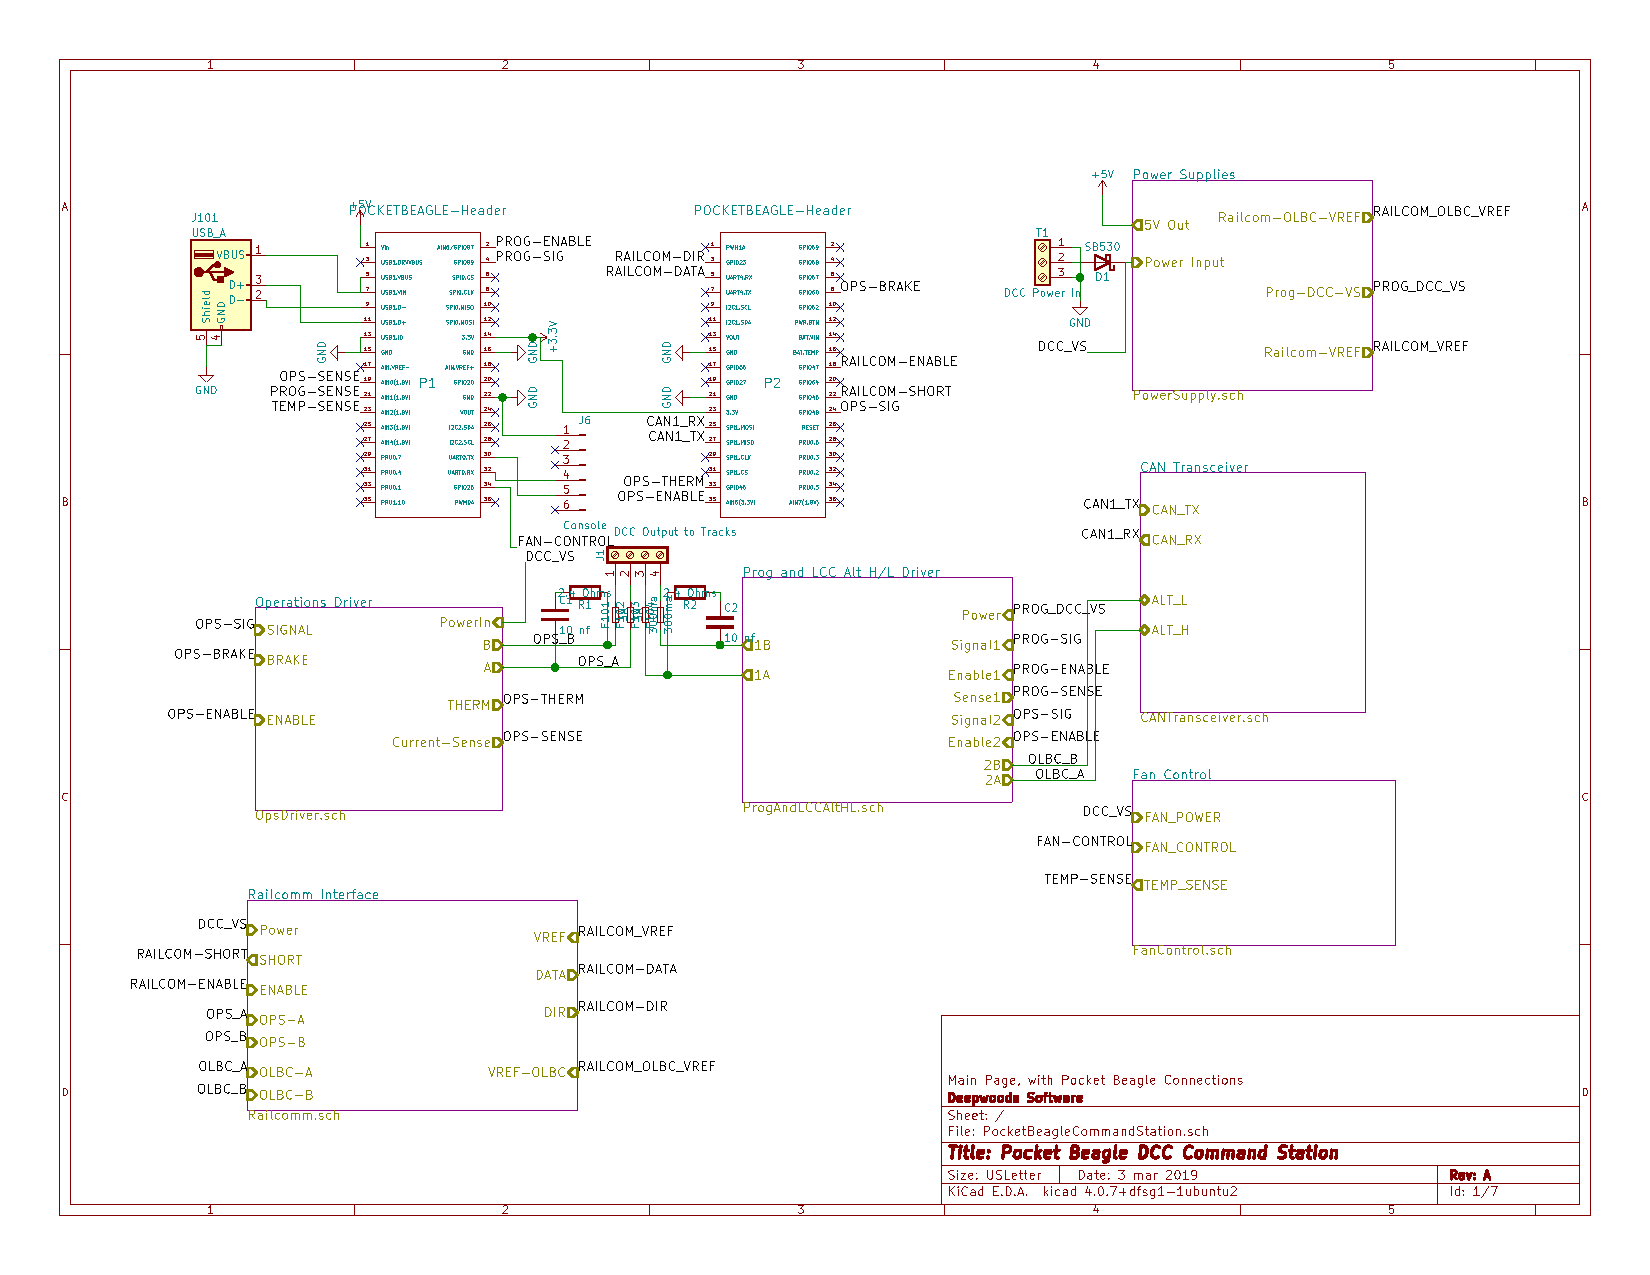
\includegraphics[width=4in]{PocketBeagleCommandStation-1.pdf}
\caption{Circuit Diagram of the PocketBeagleCommandStation board, page 1: Main 
sheet -- Section Interconnect}
\end{centering}\end{figure}
\begin{figure}[hbpt]\begin{centering}%
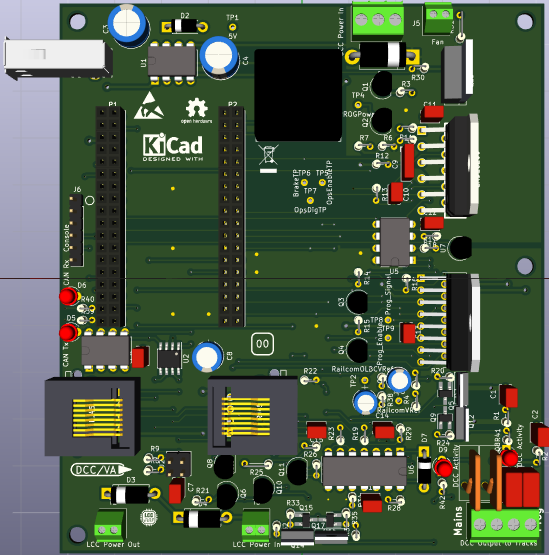
\includegraphics[width=4in]{PocketBeagleCommandStation.png}
\caption{3D Rendering of the whole board.}
\end{centering}\end{figure}

This shows how the various subsections are interconnected.
\clearpage
\subsection{Power Supplies}
\begin{figure}[hbpt]\begin{centering}%
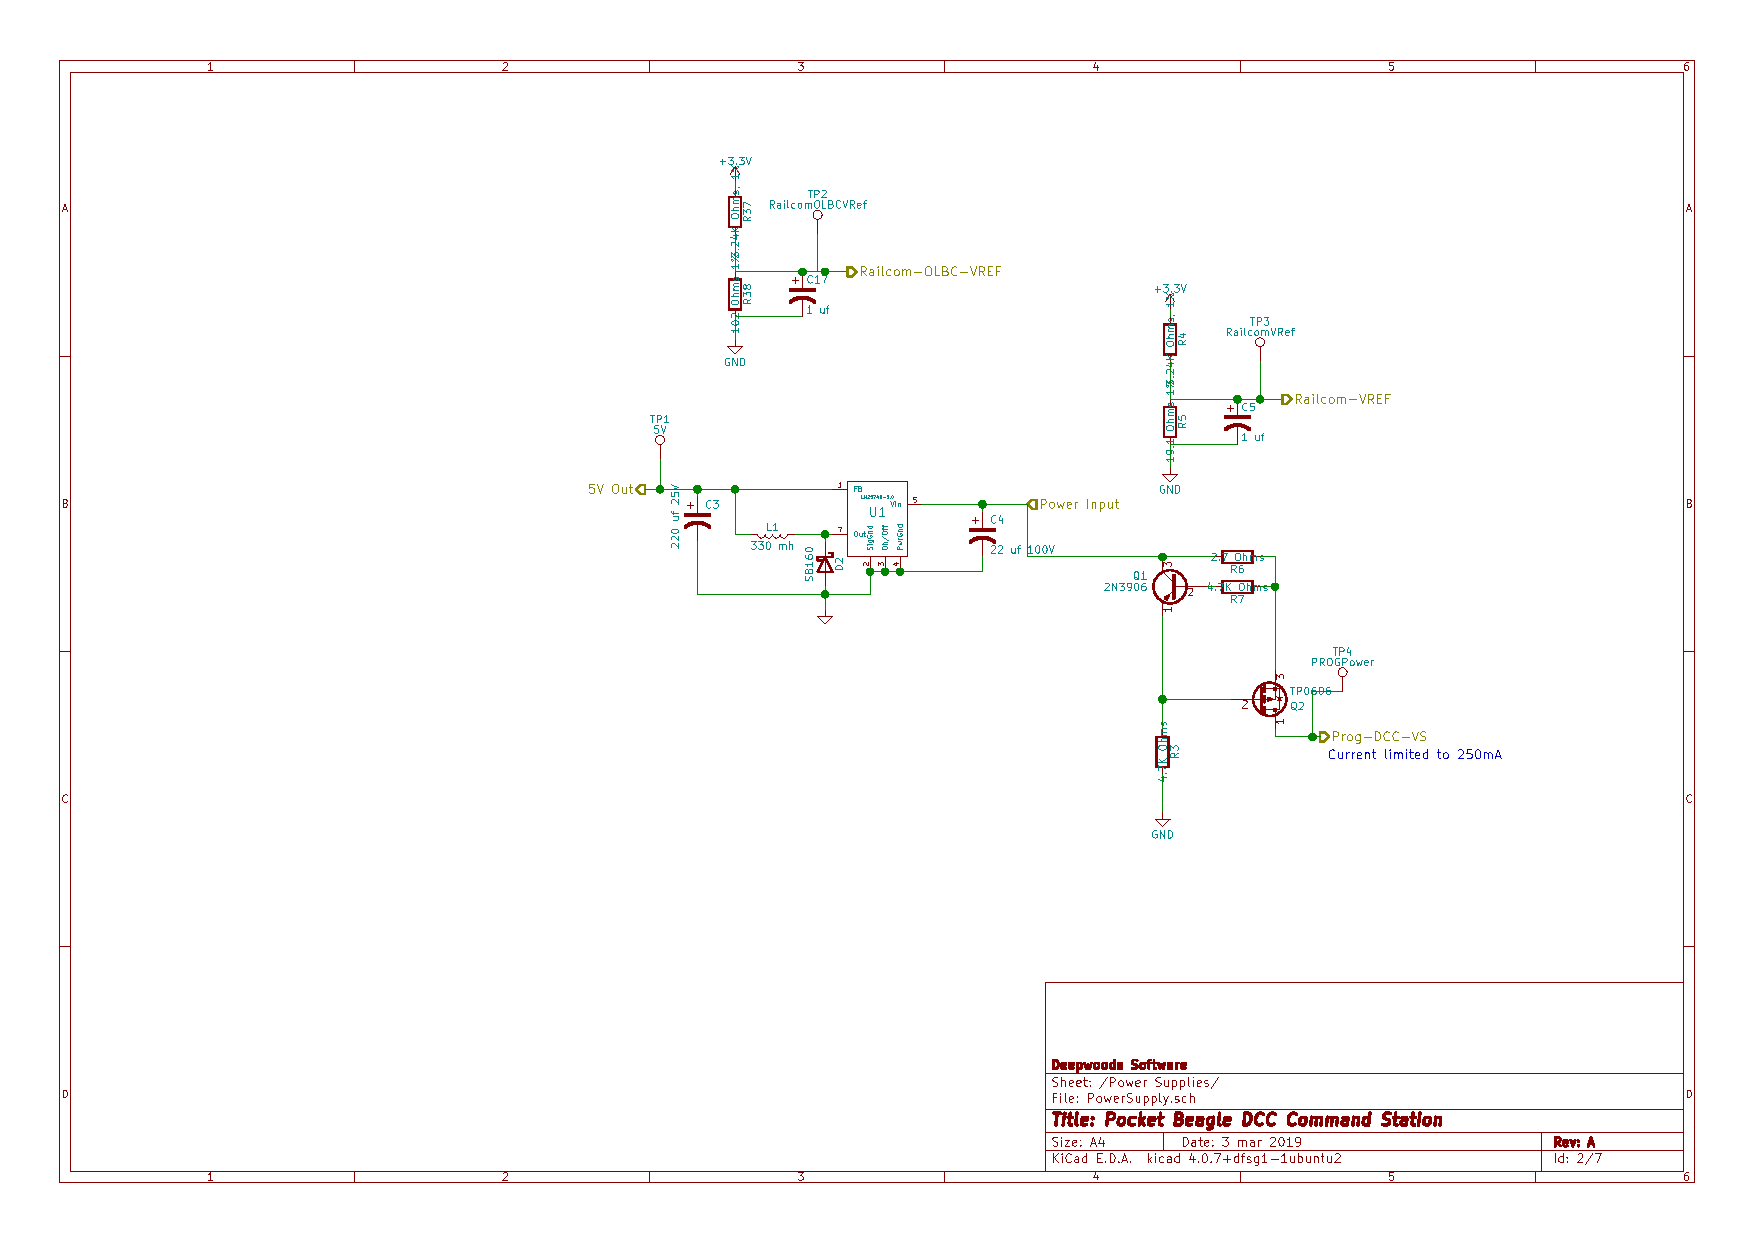
\includegraphics[width=4in]{PocketBeagleCommandStation-2.pdf}
\caption{Circuit Diagram of the PocketBeagleCommandStation board, page 2: 
Power Supplies}
\end{centering}\end{figure} 

This shows the power supply circuits.
\clearpage
\subsection{CAN Transceiver}
\begin{figure}[hbpt]\begin{centering}%
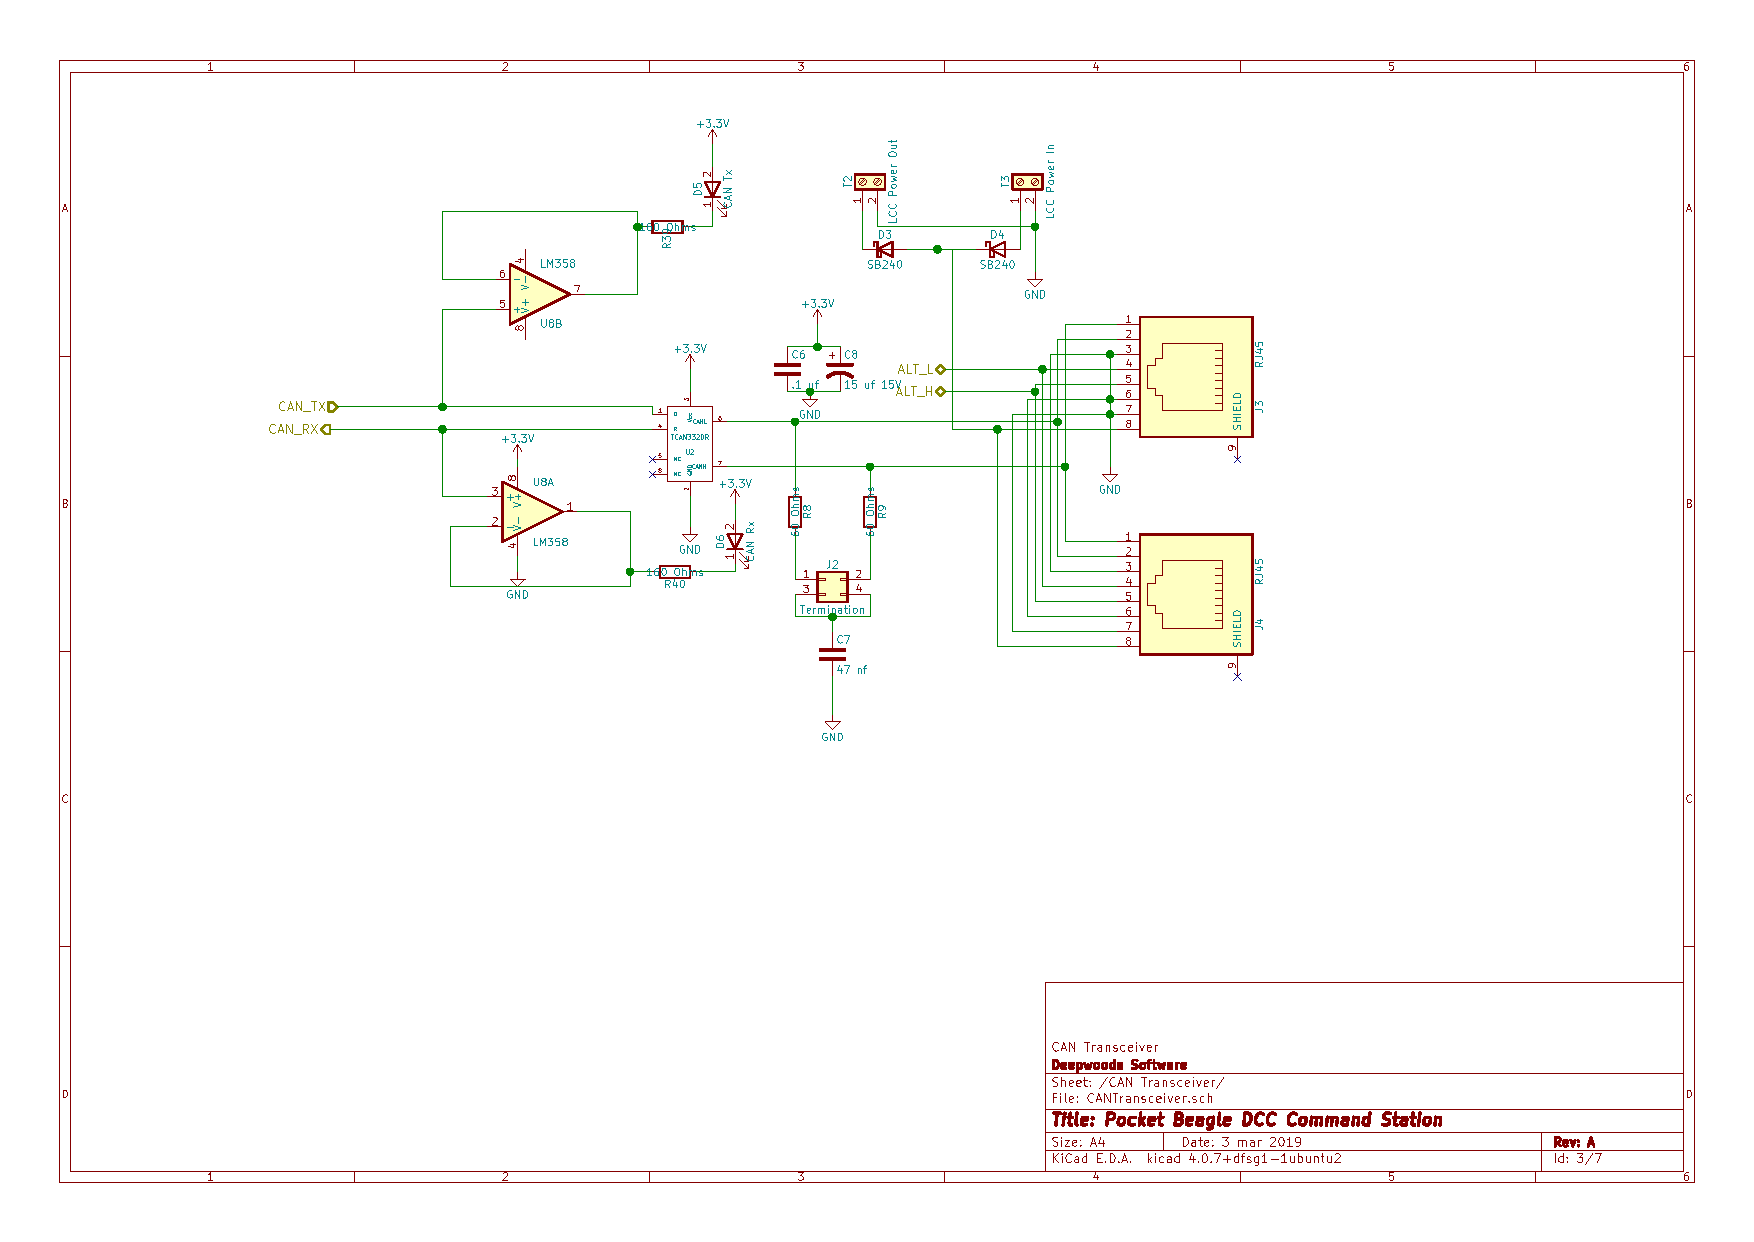
\includegraphics[width=4in]{PocketBeagleCommandStation-3.pdf}
\caption{Circuit Diagram of the PocketBeagleCommandStation board, page 3: CAN 
Transceiver}
\end{centering}\end{figure}

This shows the CAN Transceiver circuitry.
\clearpage
\subsection{OPS DCC Driver}
\begin{figure}[hbpt]\begin{centering}%
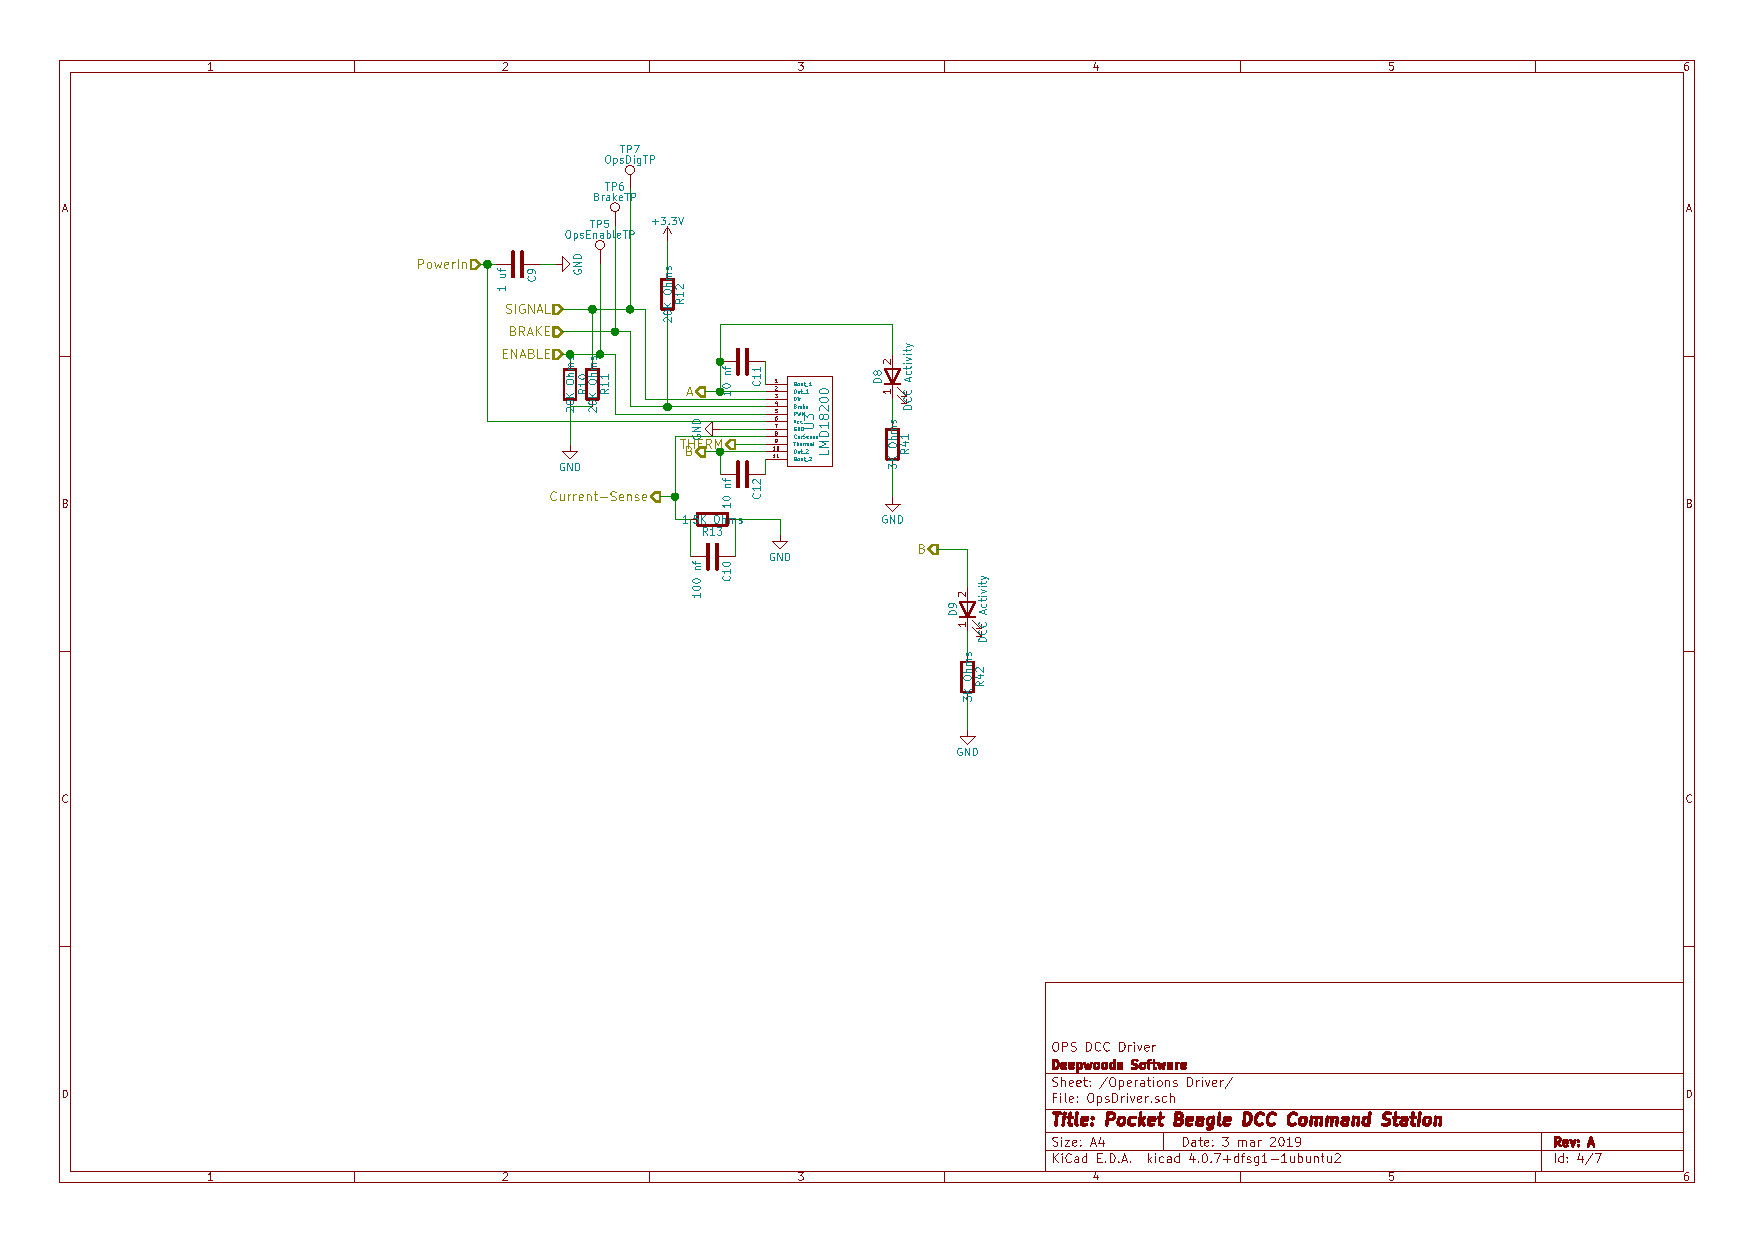
\includegraphics[width=4in]{PocketBeagleCommandStation-4.pdf}
\caption{Circuit Diagram of the PocketBeagleCommandStation board, page 4: OPS 
DCC Driver}
\end{centering}\end{figure}

This shows the OPS DCC Driver circuitry.
\clearpage
\subsection{Programming and Alt drivers}
\begin{figure}[hbpt]\begin{centering}%
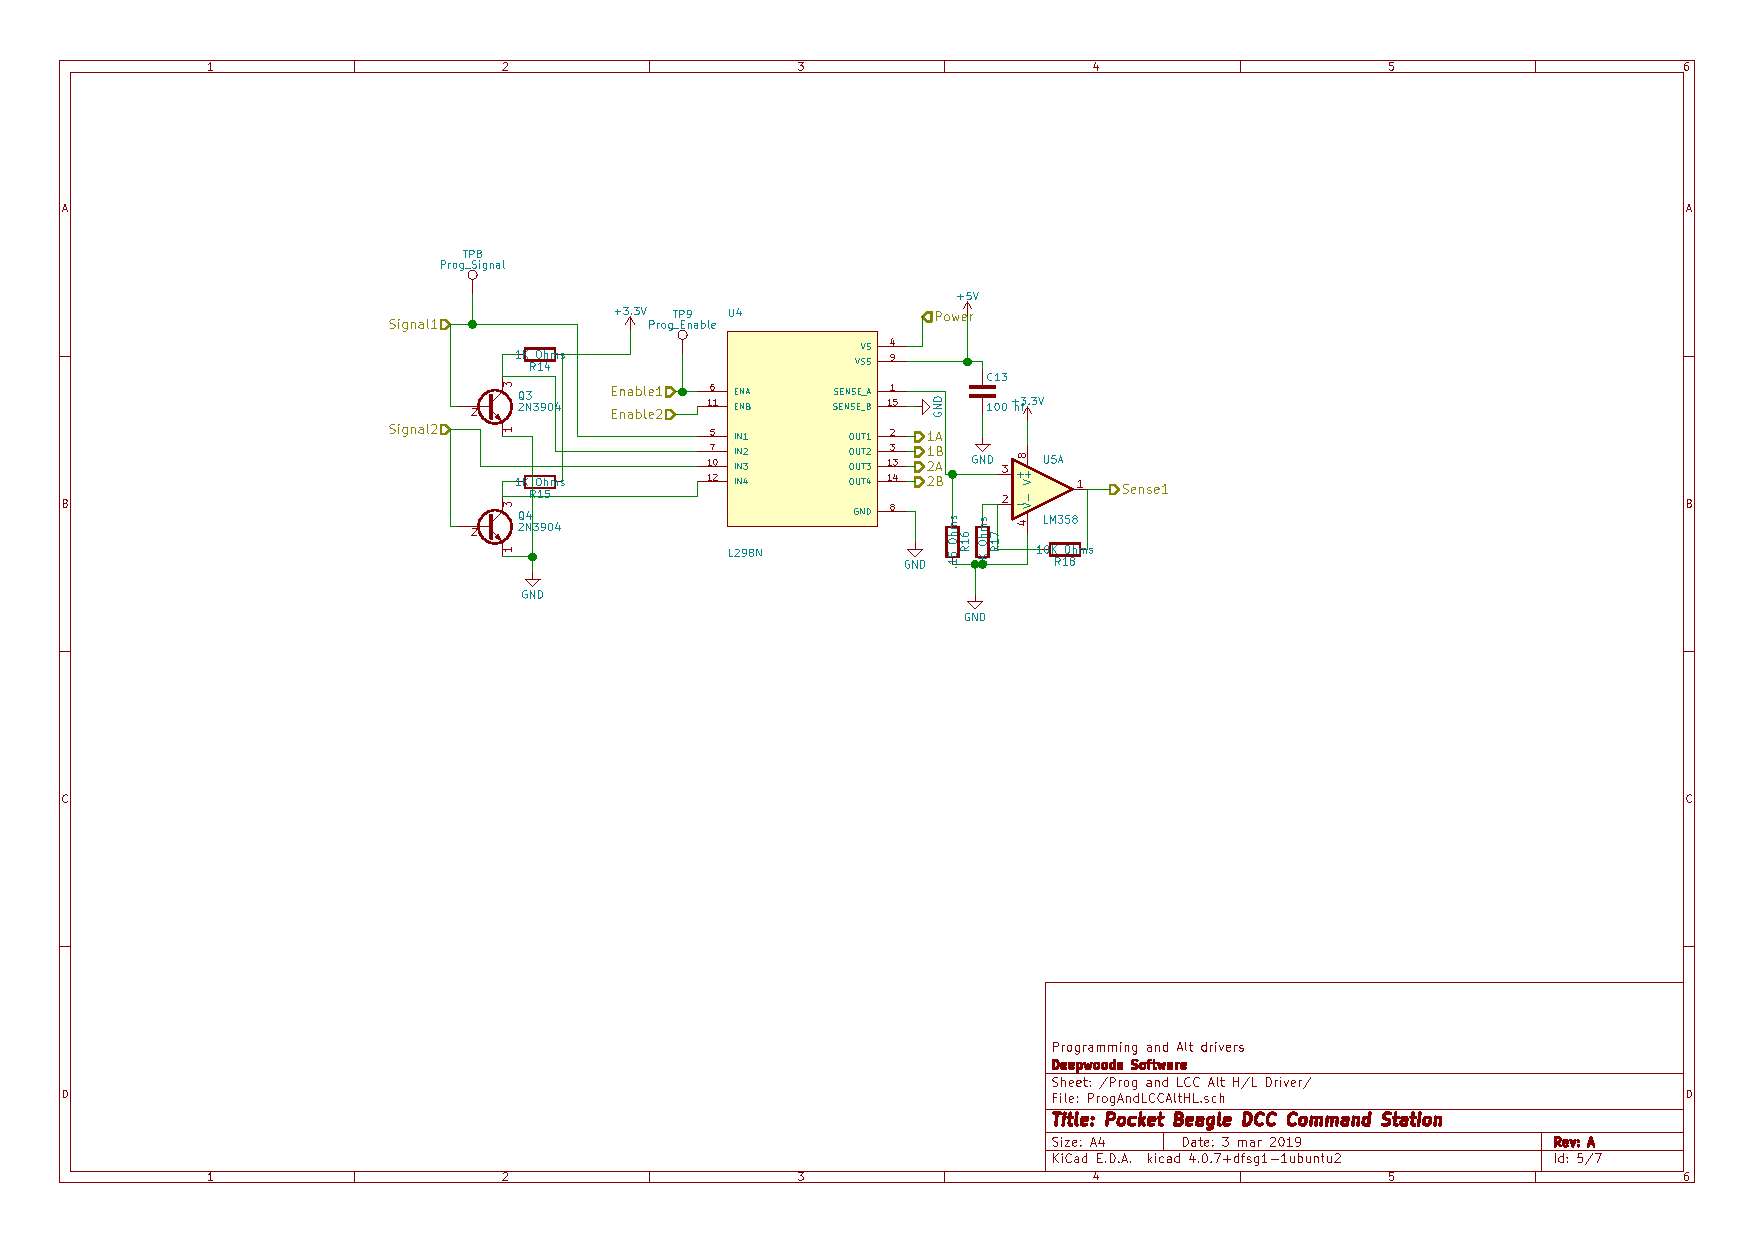
\includegraphics[width=4in]{PocketBeagleCommandStation-5.pdf}
\caption{Circuit Diagram of the PocketBeagleCommandStation board, page 5: 
Programming and Alt. DCC Driver}
\end{centering}\end{figure}

This shows the Programming and Alt. DCC Driver circuitry.
\clearpage
\subsection{Railcom Interface}
\begin{figure}[hbpt]\begin{centering}%
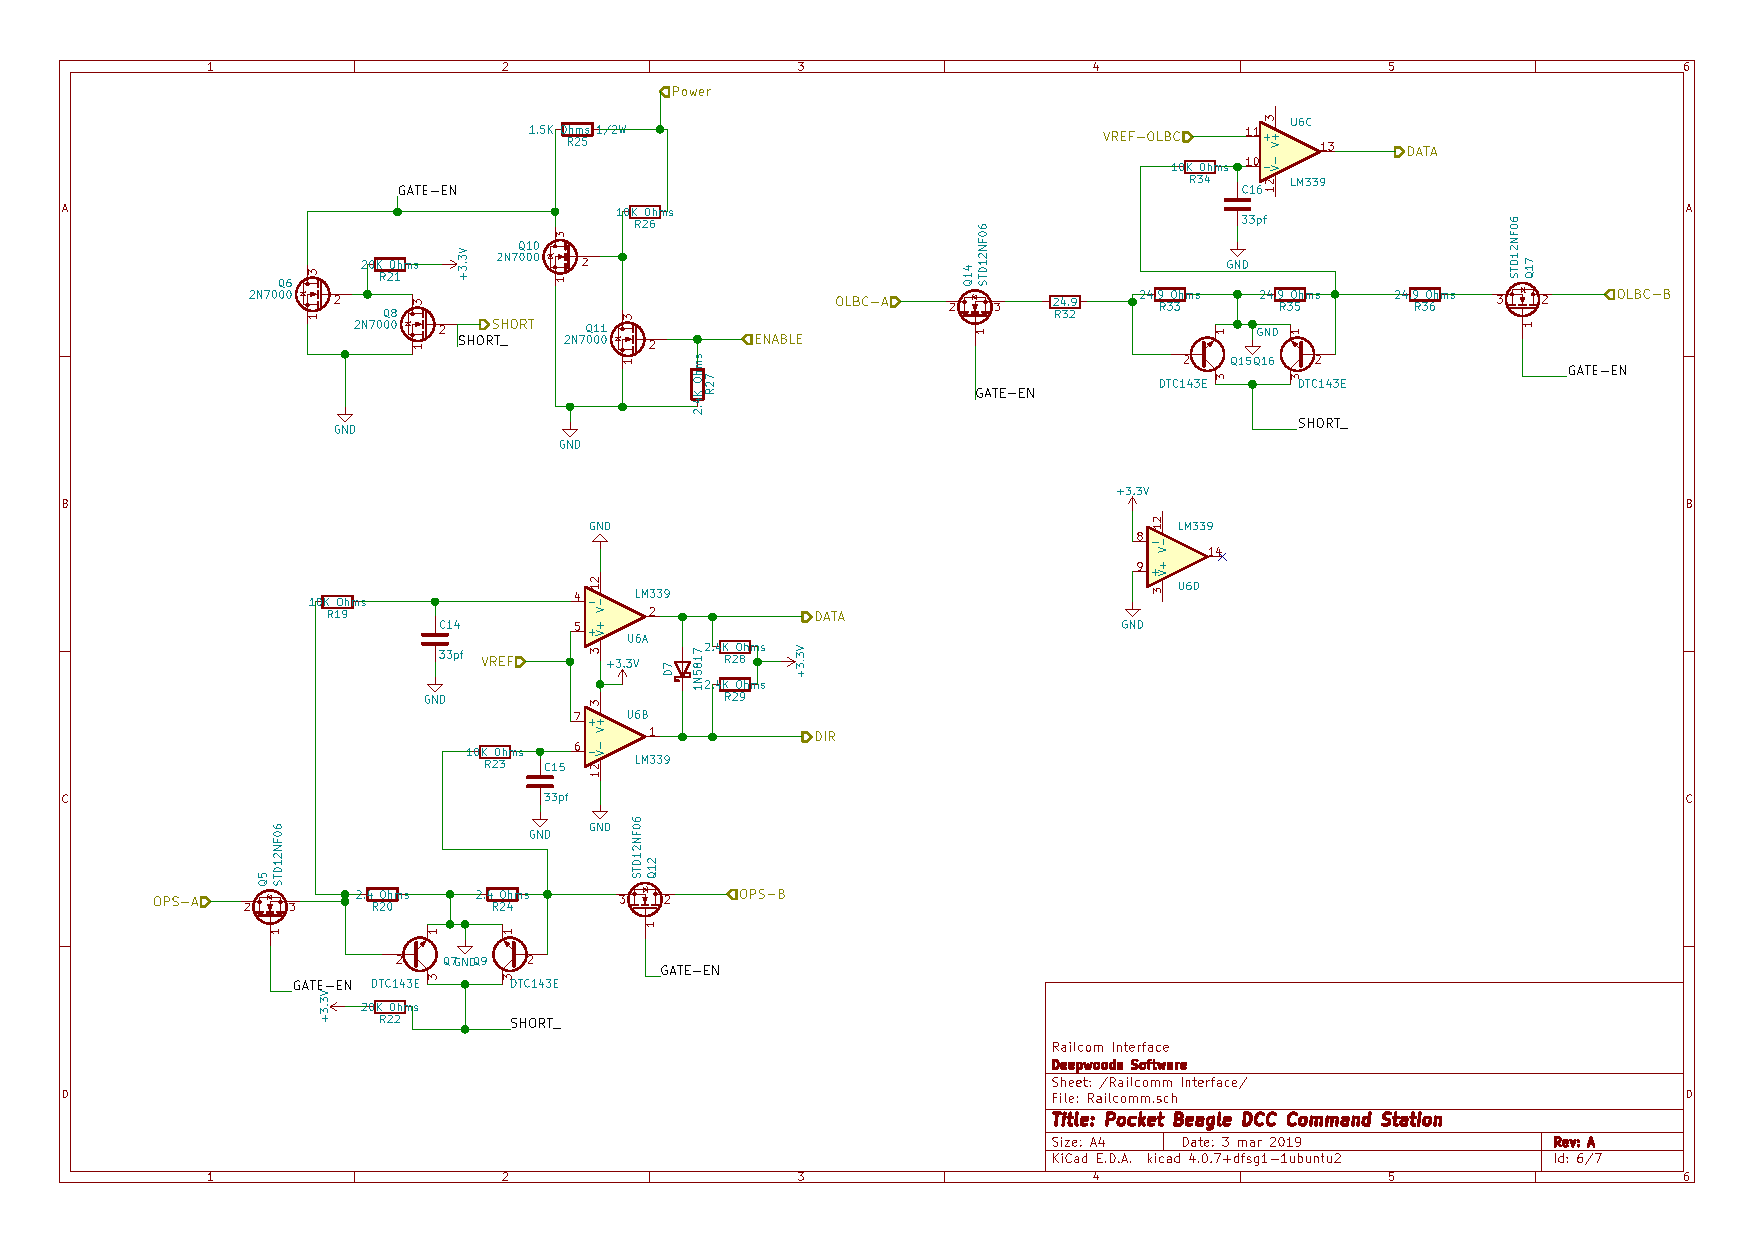
\includegraphics[width=4in]{PocketBeagleCommandStation-6.pdf}
\caption{Circuit Diagram of the PocketBeagleCommandStation board, page 6: 
Railcom Interface}
\end{centering}\end{figure}

This shows the Railcom Interface circuitry.
\clearpage
\subsection{Fan Control}
\begin{figure}[hbpt]\begin{centering}%
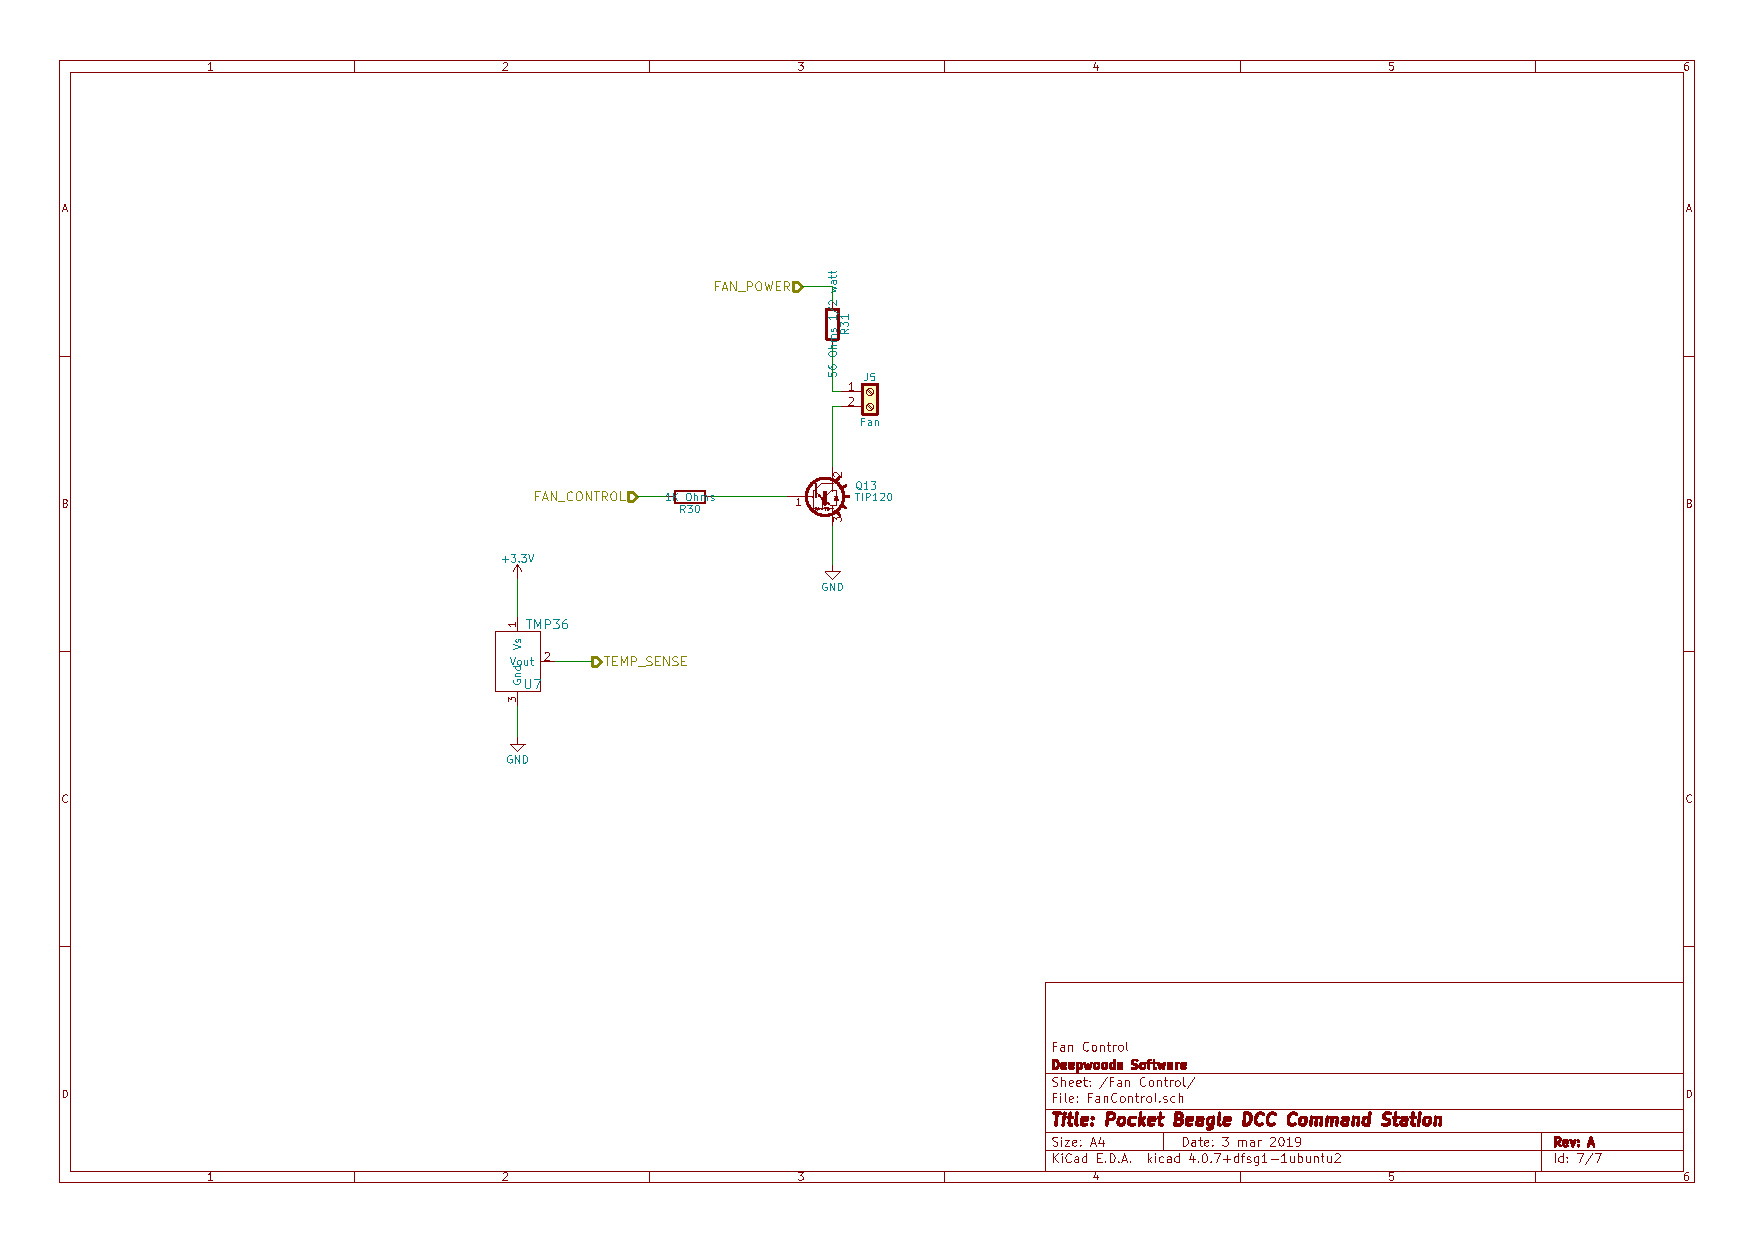
\includegraphics[width=4in]{PocketBeagleCommandStation-7.pdf}
\caption{Circuit Diagram of the PocketBeagleCommandStation board, page 7: 
Fan and temperature control}
\end{centering}\end{figure}

This shows the Fan and temperature control circuitry.
\clearpage
\section{Heatsink and Fan}
\begin{figure}[hbpt]\begin{centering}%
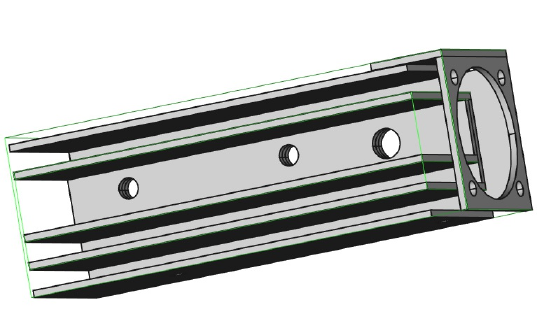
\includegraphics[width=4in]{HeatSink3D.png}
\caption{3D Rendering of the heatsink}
\end{centering}\end{figure}

A heat sink with fan can be added.  There is a temperature sensor to sense the 
temperature of the heat sink and there is a terminal block for the fan.

%\clearpage
\section{General Wiring Notes}

Wiring the Command Station is pretty straight forward. Near the upper right
corner of the PCB are two terminal blocks, a smaller 2 terminal one and a
larger 3 terminal one. The smaller one is for the fan (12VDC out) and the
larger is the power input (15VDC @ 3Amp).  The fan terminal block's terminal 
closest to the corner is the positive terminal.  The center terminal of the 
power input terminal is positive and the two outer terminals are negative (one 
of these can be used as system common/ground).

At the bottom right is a terminal block for the output to the tracks.  Two 
terminal screws for the programming track and two for the mains.

At the bottom near the left side are terminal blocks for the LCC power bus.  
This is where the termination jumper is located.

On the left side is a 6 position header for a TTY console and at the upper 
left is a female USB A (2.0) host connector.  A USB Ethernet or USB WiFi 
dongle can be plugged in here.

\section{Configuration}

The CDI for the Command Station includes the event ids for short detected and 
cleared, H-Bridge Shutdown and H-Bridge Shutdown Cleared, and thermal overload 
flag on and off for both the mains and the programming track.  There are 
temperature settings for both the alarm events and the fan, along with events 
for fan on and off.  The Command Station itself consumes no events only 
produces the above listed events.

The command station creates virtual LCC nodes for decoders and these LCC nodes 
have their own CDI's that map to CVs on the decoders.

\section{WiThrottle}

The Command Station starts a WiThrottle server, which is available if the 
command station is connected to a network with WiFi (eg there is a USB 
Ethernet or USB WiFi dongle in the USB A (2.0) host connector and is connected 
to a network).

\section{Gridconnect Hub server}

The Command Station can optionally start a Gridconnect Hub server to allow LCC 
nodes (like WiFi LCC throttles) to connect to the LCC network.

\section{Command Station ``console'' interface.}

The Command Station starts a Tcp/IP console server on port 9900 and listens
for connections. This server is a simple text-based command-line interface
meant to connect to the (separate) GUI program. Generally a PocketBeagle is
not really a powerful enough system to run a GUI. A separate computer (such as
a Raspberry Pi or really any desktop or laptop) can run the GUI program that
is available. This is not needed for the Command Station to work. While the
simple text-based command-line interface could be used directly, it is not
really meant for human interface.

\section{PocketBeagle logon}

There is a TTY serial console connector that can be used to connect to the 
PocketBeagle and then used to configure and administrate the PocketBeagle. The 
PocketBeagle is also running the SSH server and can be connected to via the 
network, either via a  USB Ethernet or USB WiFi dongle or as 192.168.6.2 or 
192.168.7.2 via its Micro-USB connector (Tcp/Ip over USB).  The default 
username:password is [debian:temppwd].

\section{Software}

The PocketBeagle runs the Linux operating system and runs the 
BBBCommandStationOpenMRN program. This through-hole PocketBeagle version uses 
the pb.linux.armv7a target.  This code alone with the OpenMRN package it 
depends on is included on the MicroSD card.  There are build configuration 
options in the Hardware.hxx in the pb.linux.armv7a target directory.  The 
built program also has run-time settings in the form of command line options. 
This is all described in the separate software manual. 

\end{document}
